% ltex: language=it
\chapter{Linguaggi Regolari}\label{chap:linguaggi_regolari} % (fold)
\section{Concetti di Base}\label{sec:lr_concetti_di_base} % (fold)
\begin{definition}{Alfabeto}{}
    Insieme finito e non vuoto di simboli.
    \begin{itemize}
        \item \textbf{binario}: $\Si = \pg{0,1}$
        \item lettere: $\Si = \pg{a,b,c,\dots,z}$
        \item insieme di tutti i caratteri ASCII
    \end{itemize}
\end{definition}
\begin{definition}{Stringa}{}
    Sequenza finita di simboli da un \textbf{alfabeto} $\Si$.
    \begin{example}{}{}
        $0011001$ è una stringa su un alfabeto $\pg{0,1}$
    \end{example}
\end{definition}
\begin{definition}{Singoletto}{}
    Un insieme di un elemento si definisce \textbf{singoletto}.
\end{definition}
\begin{definition}{Stringa Vuota}{}
    La \textbf{stringa} con zero occorrenze di simboli da $\Si$.
    \begin{note}
        La stringa vuota è denotata con $\eps$
    \end{note}
\end{definition}
\begin{definition}{Linghezza di una stringa}{}
    Numero di posizioni per i simboli nella stringa.
    $\ab{w}$ denota la lunghezza della stringa $w$
\end{definition}
\begin{definition}{Potenze}{}
    La \textbf{potenza} di un alfabeto si denota con $\Si[k]$ e corrisponde all'insieme delle stringhe di lunghezza $k$ con simboli da $\Si$
    \begin{itemize}
        \item $\Si = \pg{0,1}$
        \item $\Si[1] = \pg{0,1}$
        \item $\Si[2] = \pg{00, 01, 10, 11}$
        \item $\Si[0] = \pg{\eps}$
    \end{itemize}
\end{definition}
\begin{note}
    L'inseme di tutte le stringhe su $\Si$ è denotato da $\Si[*]$
    \[
        \Si[+] = \Si[1] \cup\Si[2] \cup  \Si[3] \cup\dots
    \]
    \[
        \Si[*] = \Si[+] \cup \pg \eps
    \]
\end{note}
\begin{definition}{Concatenzazione}{}
    Se $x$ e $y$ sono stringhe, allora $xy$ è la stringa ottenuta collocando una copia di $y$ subito dopo una copia di $x$.
    \[
        \begin{aligned}
            &x = a_1a_2\,\dots\,a_i \qquad y = b_1b_2\,\dots\,b_j \\
            &xy = a_1a_2\,\dots\,a_ib_1b_2\,\dots\,b_j
        \end{aligned}
    \]
    \begin{note}
        Per ogni stringa $x$:
        \[
            x\eps = \eps x = x
        \]
    \end{note}
\end{definition}
\begin{definition}{Linguaggi formali}{}
    Se $\Si$ è un alfabeto, e $L \subseteq \Si[*]$ allora $L$ è un \textbf{linguaggio formale}
    \begin{note}[Linguaggio Vuoto]
        \[
            \emptyset
        \]
        Il linguaggio vuoto è diverso da $\pg{\eps}$
    \end{note}
\end{definition}
% section Concetti di Base (end)
%
\subsection{Automi a Stati Finiti Deterministici}\label{sub:lr_automi_a_stati_finiti_deterministici} % (fold)
Un \ac{dfa} è una \textbf{quintupla}:
\[
    A = \pt{Q,\Si,\dt, q_0, F}
\]
\begin{itemize}
    \item $Q$ è un insieme \textbf{finito di stati};
    \item $\Si$ è un alfabeto finito;
    \item $\dt$ è una funzione di transizione da $Q\times \Si$ a $Q$, cioè: $\pt{q,a}\mapsto p$ (solo in un certo stato leggo un simbolo);
    \item $q_0 \in Q$ è lo stato iniziale;
    \item $F \subseteq Q$ è un insieme di stati \textbf{finali} (stati di accettazione);
\end{itemize}
\begin{critical}
    Per ogni stato deve essere presente una e una sola transizione uscente etichettata per ogni lettera dell'alfabeto.
    \emptyln{}
    Nell'esempio \cref{ex:first-ex} lo stato $q_0$ non può avere due transizioni con etichetta $1$ e non può mancare la transizione con l'etichetta $1$.
\end{critical}
\begin{example}{Un automa A che accetta $L=\pg{x01y: x,y \in \pg{0,1}^*}$}{first-ex}
    L'automa $A = \pt{\pg{q_0,q_1,q_2},\pg{0,1},\dt,q_0,\pg{q_1}}$ definito tramite una \textbf{tabella di transizione}:
    \begin{ctable}{r||c|c}
        & 0 & 1 \\
        \midrule
        \midrule
        $\rightarrow q_0$ & $q_2$ & $q_0$ \\
        $\star q_1$       & $q_1$ & $q_1$ \\
        $q_2$             & $q_2$ & $q_1$ \\
    \end{ctable}
    Lo stesso automa $A$ può essere definito tramite un \textbf{diagramma di transizione}:
    \begin{cimage}
        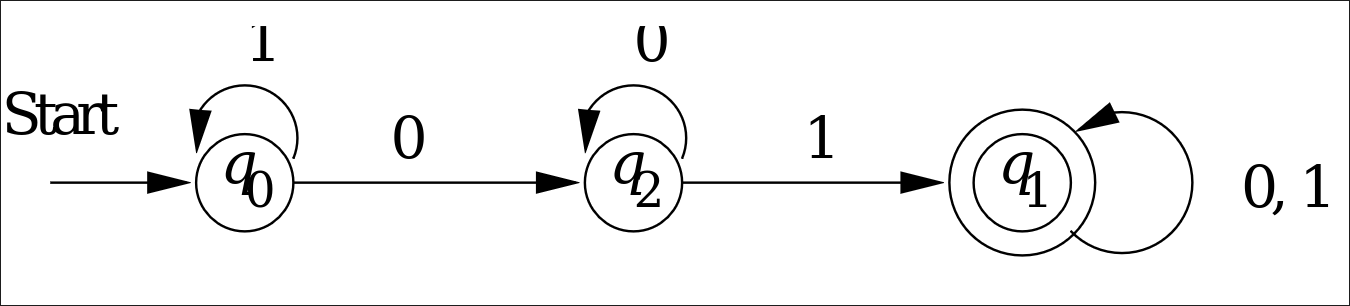
\includegraphics[width=.8\textwidth]{assets/dfa-ex-diag.png}
    \end{cimage}
\end{example}
Un automa a stati finiti accetta una stringa $w = a_1a_2\cdots a_n$ se esiste un cammino nel diagramma di transizione che:
\begin{enumerate}
    \item inizia nello \textbf{stato iniziale};
    \item finisce in uno \textbf{stato finale};
    \item ha una \textbf{sequenza} di etichette $a_1a_2\cdots a_n$;
\end{enumerate}
\begin{note}[Estensione Funzioni di Transizione]
    La \textbf{funzione d transizione} $\dt$ può essere estesa a $\hat\dt$ che opera su stati e stringhe, invece che su stati e simboli.
    \begin{description}
        \item[Base] $\hat\dt\pt{q,\eps} = q$
        \item[Induzione] $\hat\dt\pt{q,xa} = \dt\pt{\hat\dt\pt{q,x}a}$
    \end{description}
    Formalmente \hyperref[def:ling-reg]{il linguaggio accettato da un automa} a stati finiti deterministico $A$ è:
    \[
        L\pt A = \pg{w : \hat\dt\pt{q-0,w} \in F}
    \]
\end{note}
\begin{definition}{Linguaggi Regolari}{ling-reg}
    Tutti i linguaggi accettati da automi a stati finiti sono detti \textbf{linguaggi regolari}
\end{definition}
\begin{example}{Funzione di Transizione Induttiva}{}
    \begin{cimage}
        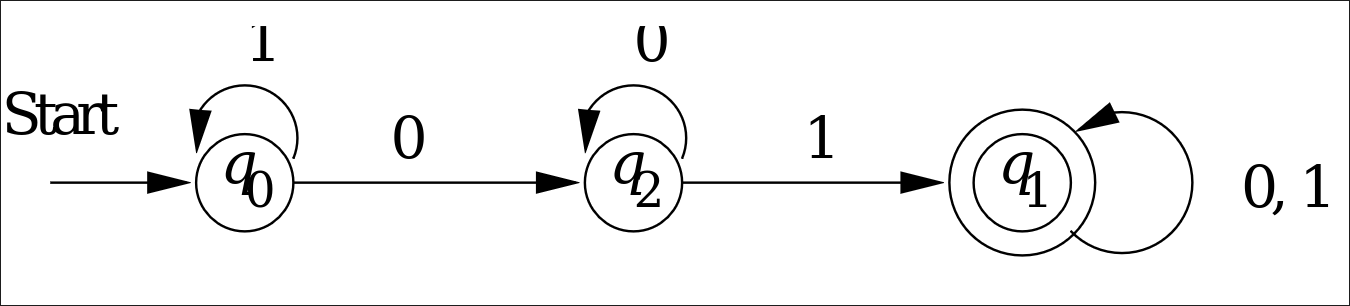
\includegraphics[width=.8\textwidth]{assets/dfa-ex-diag.png}
    \end{cimage}
    \begin{description}
        \item[Base] $\hat\dt\pt{q,\eps} = q$
        \item[Induzione] $\hat\dt\pt{q,xa} = \dt\pt{\hat\dt\pt{q,x}a}$
    \end{description}
    Calcoliamo $\hat\dt\pt{q_0,0110}$
    \[
        \begin{aligned}
            &\hat\dt\pt{q_0,\eps} = q_0 \\
            &\hat\dt\pt{q_0, \red{\eps}0} = \dt\pt{\underbrace{\hat\dt\pt{q_0,\eps}}_{\red{q_0}}, 0} = \dt\pt{q_0, 0} = \red{q_2} \\
            &\hat\dt\pt{q_0, \red{0}1} = \dt\pt{\underbrace{\hat\dt\pt{q_0,0}}_{\red{q_2}}, 1} = \dt\pt{q_2, 1} = \red{q_1} \\
            &\hat\dt\pt{q_0, \red{01}1} = \dt\pt{\underbrace{\hat\dt\pt{q_0,01}}_{\red{q_1}}, 1} = \dt\pt{q_1, 1} = \red{q_1} \\
            &\hat\dt\pt{q_0, \red{011}0} = \dt\pt{\underbrace{\hat\dt\pt{q_0,011}}_{\red{q_1}}, 0} = \dt\pt{q_1, 0} = \red{q_1} \\
        \end{aligned}
    \]
\end{example}
% subsection Automi a Stati Finiti Deterministici (end)
% chapter Linguaggi Regolari (end)
